\chapter{Interferometric methods in tokamak plasmas}


\section{Gaussian beam diffraction}


\subsection{Definition of a Gaussian beam}
A Gaussian beam of angular frequency $\omega_0$
propagating along the $z$-axis
has an electric field
\begin{equation}
  E(\vect{r}, t)
  =
  E_G(\vect{r}) e^{-i \omega_0 t}
\end{equation}
with spatial dependence~\cite{siegman_lasers}
\begin{equation}
  E_G(\vect{r})
  =
  E_0
  \frac{w_0}{w(z)}
  \exp\left[ \frac{-\rho^2}{w(z)^2} \right]
  \exp\left\{ i \left[
    k_0 z
    +
    \frac{k_0 \rho^2}{2 R(z)}
    -
    \psi(z) \right] \right\}
  \label{eq:InterferometricMethods:Gaussian_beam}
\end{equation}
Here,
$\rho = (x^2 + y^2)^{1/2}$ is the transverse distance from the optical axis,
$w_0$ is the radius of the beam's waist, and
$k_0 = \omega_0 / c = 2 \pi / \lambda_0$ is the beam's wavenumber.
The beam's width $w(z)$, radius of curvature $R(z)$, and
Gouy phase $\psi(z)$ are defined as
\begin{align}
  w(z)
  &=
  w_0 \left[ 1 + \left( \frac{z}{z_R} \right)^2 \right]^{1/2}
  \label{eq:InterferometricMethods:Gaussian_beam_width}
  \\
  R(z)
  &=
  z \left[ 1 + \left( \frac{z_R}{z} \right)^2 \right]
  \label{eq:InterferometricMethods:Gaussian_beam_radius_of_curvature}
  \\
  \psi(z)
  &=
  \atan\left( \frac{z}{z_R} \right)
  \label{eq:InterferometricMethods:Gouy_phase}
\end{align}
where the Rayleigh range
\begin{equation}
  z_R \equiv \frac{\pi w_0^2}{\lambda_0}
  \label{eq:InterferometricMethods:Rayleigh_range}
\end{equation}
is the nominal division between the beam's
near-field ($|z| \ll z_R$) and far-field ($|z| \gg z_R$) behaviors.


\subsection{Kirchhoff diffraction theory}
A monochromatic scalar wave $U(\vect{r}) e^{-i \omega t}$ in vacuum
satisfies the Helmholtz equation
\begin{equation}
  (\nabla^2 + k^2) U = 0
\end{equation}
where $k = \omega / c$.
The Helmholtz-Kirchhoff integral theorem states
that the field at a point $P$ is
\begin{equation}
  U(P)
  =
  \frac{1}{4 \pi}
  \int_S \left[
    U \frac{\partial}{\partial n}\left(\frac{e^{i k s}}{s}\right)
    -
    \frac{e^{i k s}}{s} \frac{\partial U}{\partial n}
  \right] dS
  \label{eq:InterferometricMethods:Helmholtz_Kirchhoff_integral_theorem}
\end{equation}
where $S$ is an arbitrary surface that encloses $P$,
$\vect{s}$ is the vector from point $P$ to differential area element $dS$,
$\vect{n}$ is the \emph{inward}-pointing normal of surface $S$, and
$U$ is assumed to be differentiable to second order within and on $S$
\cite{born_and_wolf}.
The relevant geometry is sketched
in Fig.~\ref{fig:InterferometricMethods:Kirchhoff_geometry}(a).

\begin{figure}
  \centering
  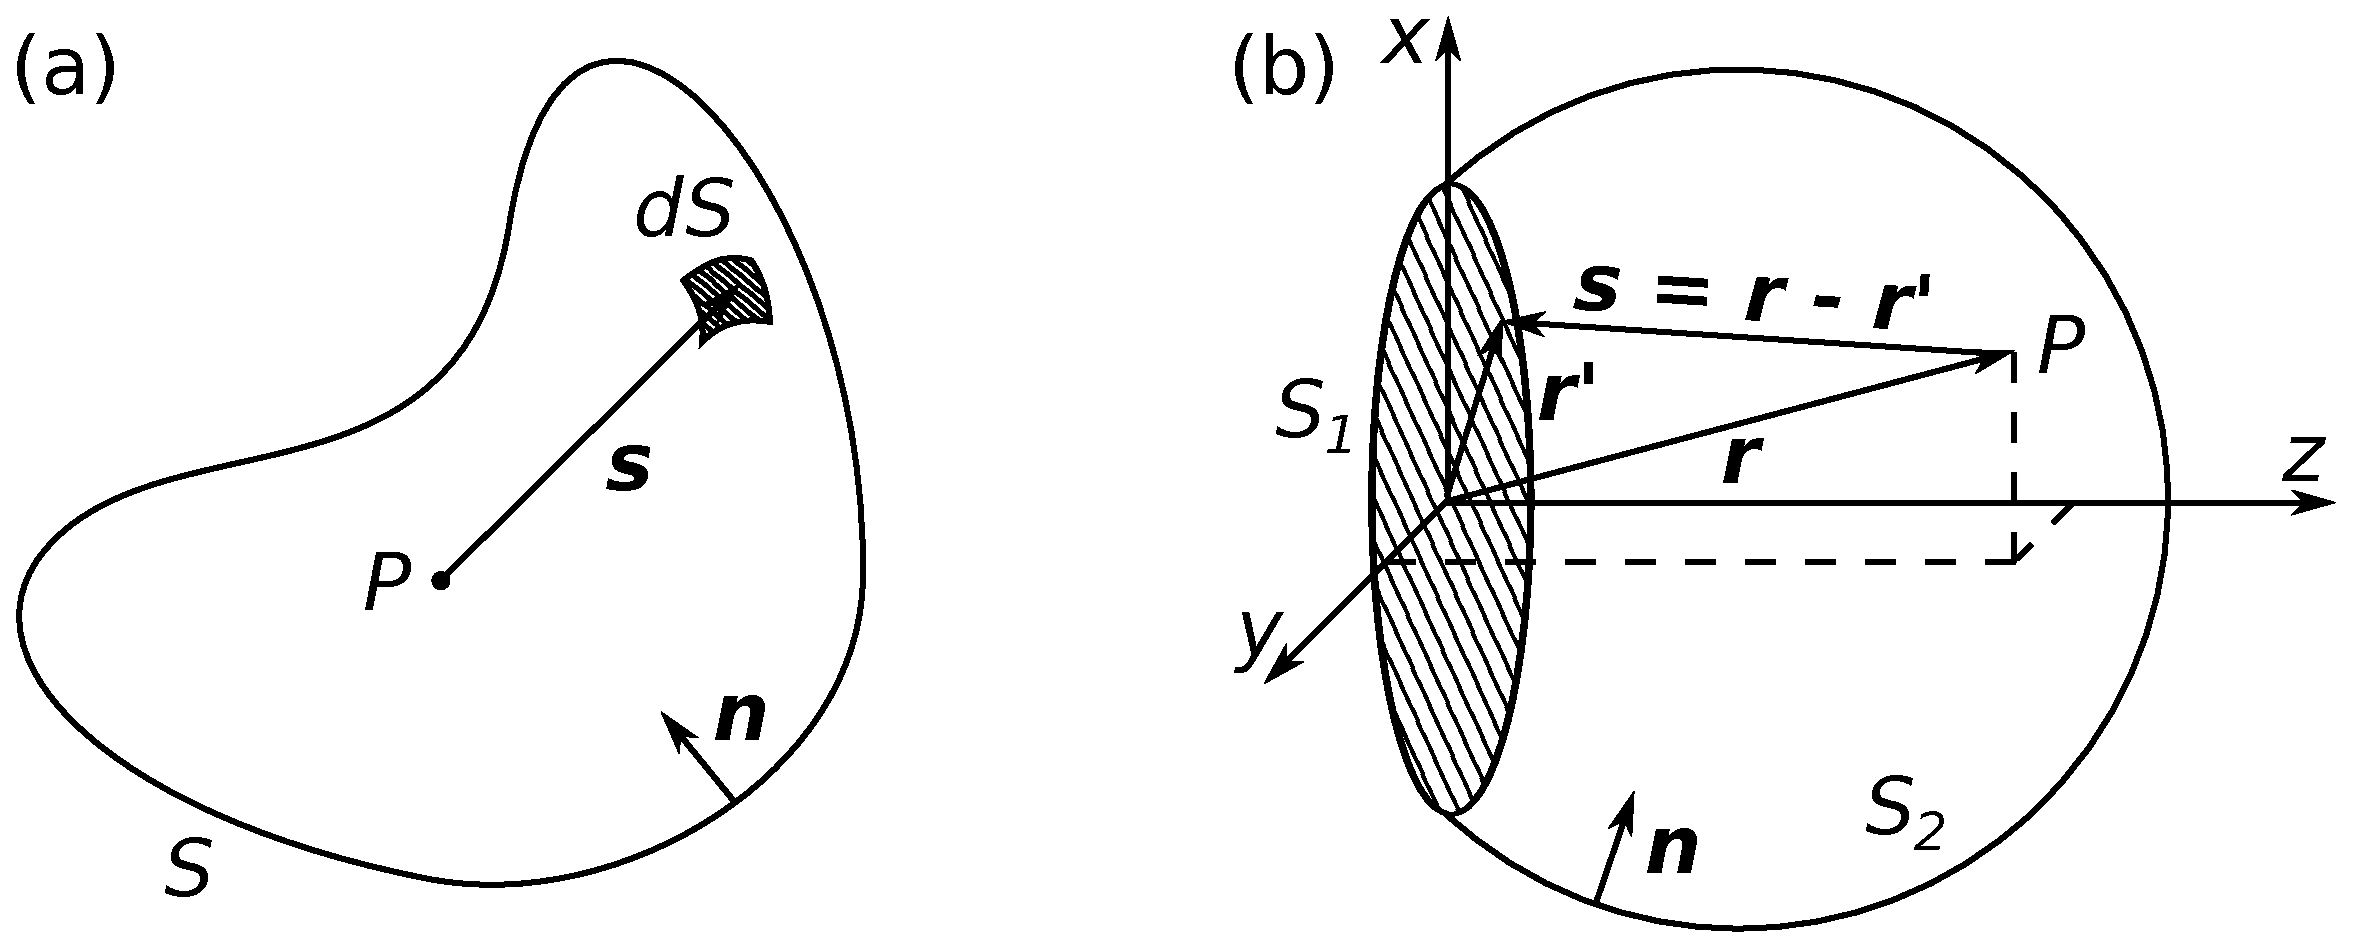
\includegraphics[width = \textwidth]{%
    Chapters/InterferometricMethods/figs/kirchhoff_geometry.eps}
  \caption{Geometries for Kirchhoff diffraction calculations}
\label{fig:InterferometricMethods:Kirchhoff_geometry}
\end{figure}

To proceed with the diffraction calculation,
assume that the incident waves propagate in the $+z$-direction and
adopt the surface drawn
in Fig.~\ref{fig:InterferometricMethods:Kirchhoff_geometry}(b).
That is, $S = S_1 + S_2$,
where $S_1$ is a circle in the $(x, y)$-plane, and
$S_2$ is a spherical segment centered on the optical axis.
Now, assume that the incident waves were ``turned on''
at some finite time in the past, and
take the radius of $S_2$ to be large enough such that
none of the diffracted waves have had sufficient time to reach $S_2$,
i.e.\ $U \equiv 0$ on $S_2$.
(Of course, strictly speaking, the source's finite turn-on time
requires relaxation of the monochromatic assumption.
Finite turn-on time does not preclude a pseudo-monochromatic source, however,
and such a source is assumed hereafter).
Thus, the integral over $S_2$ vanishes, and
(\ref{eq:InterferometricMethods:Helmholtz_Kirchhoff_integral_theorem})
reduces to an integral over $S_1$.

Evaluation of
(\ref{eq:InterferometricMethods:Helmholtz_Kirchhoff_integral_theorem})
requires knowledge of $U$ on $S_1$.
For free-space propagation,
$S_1$ is an imagined (rather than a physical) surface
that does not impede the propagation of the incident beam $U^{(i)}$
(that is, $U = U^{(i)}$ and
$\partial U / \partial n = \partial U^{(i)} / \partial n$ on $S_1$).
If, however, $S_1$ contains opaque obstacles,
the free-space propagation conditions are no longer valid;
instead, the Kirchhoff boundary conditions can be adopted:
\begin{align}
  \text{surfaces of clear aperture:}&
  \quad
  U = U^{(i)},
  \quad
  \frac{\partial U}{\partial n} = \frac{\partial U^{(i)}}{\partial n}
  \\
  \text{opaque surfaces:}&
  \quad \;
  U = 0,
  \qquad
  \frac{\partial U}{\partial n} = 0
\end{align}
While these boundary conditions are adequate for the current application,
it should be noted that they are not physical
for points that are very close to the boundaries of the opaque obstacles.


\subsection{Fraunhofer diffraction of a free-space Gaussian beam}
Assume that the incident Gaussian beam has a waist at $S_1$, and
take the radius of $S_1$ to be much larger than the beam waist $w_0$
such that the domain of integration effectively extends
over the whole $(x, y)$-plane.
For free-space propagation,
$S_1$ does not perturb the Gaussian beam; thus,
$E(\vect{r}, t) = E^{(i)}(\vect{r}, t) = E_G(\vect{r}) e^{-i \omega_0 t}$.
Now, in the far-field ($k_0 s \gg 1$) and
paraxial ($\vect{s} \approx -z \hat{\vect{z}}$) approximations
\begin{align}
  \left. \frac{e^{i k_0 s}}{s} \right|_{S_1}
  &\approx
  \frac{e^{i k_0 s}}{z}
  \\
  \left. \frac{\partial}{\partial n}
  \left( \frac{e^{i k_0 s}}{s} \right) \right|_{S_1}
  &\approx
  -i k_0 \left( \frac{e^{i k_0 s}}{z} \right)
\end{align}
The $s$-dependence in the phase arguments has been retained,
as it is the mechanism responsible for diffraction, but
the $s$-dependence in the amplitude has been dropped
as it only gives rise to negligible variations
in the amplitude of the diffracted wave.
Relative to a spherical wave,
a Gaussian beam has several additional $z$-dependencies;
however, at the beam's waist
\begin{align}
  \left. \frac{\partial w(z)}{\partial z} \right|_{\text{waist}}
  &\equiv
  0
  \\
  \left. \frac{\partial}{\partial z}
  \left[ \frac{1}{R(z)} \right] \right|_{\text{waist}}
  &=
  \frac{1}{z_R^2}
  \\
  \left. \frac{\partial \psi(z)}{\partial z} \right|_{\text{waist}}
  &=
  \frac{1}{z_R}
\end{align}
Then, if the beam's Rayleigh range is much greater than
the probe wavelength ($k_0 z_R \gg 1$) and
the relevant transverse dimensions are much less than
the Rayleigh range ($w_0 \ll z_R$),
the Gaussian beam at $S_1$ satisfies
\begin{align}
  \left. E_G(\vect{r'}) \right|_{S_1}
  &\approx
  E_0 e^{-(\rho' / w_0)^2}
  \\
  \left. \frac{\partial E_G(\vect{r'})}{\partial n} \right|_{S_1}
  &\approx
  i k_0 \left[ E_0 e^{-(\rho' / w_0)^2} \right]
\end{align}
Note that the CO$_2$ laser beams ($k_0 \approx \SI{2 \pi e5}{\per\meter}$)
that probe tokamak plasmas often have $z_R \gg \SI{10}{\meter}$
such that $k_0 z_R \gg 1$ and $w_0 \ll z_R$
(the transverse dimensions are constrained by the machine size
such that $w_0 \ll \SI{1}{\meter}$) are very well satisfied.

Substituting the above expressions for
the incident waves and their surface-normal derivatives into
(\ref{eq:InterferometricMethods:Helmholtz_Kirchhoff_integral_theorem})
and simplifying yields
\begin{equation}
  E(\vect{r})
  \approx
  \frac{-i E_0}{\lambda_0 z}
  \int_{S_1}
  e^{-( \rho' / w_0 )^2}
  e^{i k_0 s}
  dS
  \label{eq:InterferometricMethods:Kirchhoff_diffraction_integral}
\end{equation}
To proceed further, $s$ must be approximated:
\begin{align}
  s
  &=
  | \vect{r'} - \vect{r}|
  \notag \\
  &=
  \left[ r^2 - 2(x'x + y'y) + (x'^2 + y'^2) \right]^{1/2}
  \notag \\
  &\approx
  r - \frac{x'x + y'y}{r}
  \label{eq:InterferometricMethods:Fraunhofer_s}
\end{align}
where only terms linear in $(x' / r)$ and $(y' / r)$ have been retained.
This is known as the Fraunhofer limit, and
it is valid for $z \gg z_R$~\cite{born_and_wolf}.
Under the Fraunhofer limit
(\ref{eq:InterferometricMethods:Kirchhoff_diffraction_integral}) becomes
\begin{equation}
  E(\vect{r})
  \approx
  \frac{-i E_0}{\lambda_0 z}
  e^{i k_0 r}
  D_x D_y
  \label{eq:InterferometricMethods:Fraunhofer_diffracted_field}
\end{equation}
where
\begin{equation}
  D_x
  =
  \int_{-\infty}^{\infty}
  e^{-( x' / w_0 )^2}
  e^{-i k_0 x x' / r}
  dx'
  \label{eq:InterferometricMethods:Fraunhofer_diffraction_integral_free_space}
\end{equation}
gives the diffraction pattern in the $x$-direction, and
replacing $x$ with $y$ in
(\ref{eq:InterferometricMethods:Fraunhofer_diffraction_integral_free_space})
yields the expression for the diffraction pattern in the $y$-direction, $D_y$.
Note that the $e^{-i k_0 x x' / r} = e^{-i k_0 x' \sin\theta}$ term
is the typical geometric phase factor
of interference and diffraction calculations
that results from path-length differences between
points on surface $S_1$ and the field point $\vect{r}$, as shown in
Fig.~{\ref{fig:InterferometricMethods:Fraunhofer_geometric_phase_factor}}.
Eq.~(\ref{eq:InterferometricMethods:Fraunhofer_diffraction_integral_free_space})
is easily evaluated, as it is simply the Fourier transform of a Gaussian
\begin{equation}
  D_x
  =
  \sqrt{\pi} w_0 e^{-(k_0 w_0 x / 2 r)^2}
\end{equation}
and (\ref{eq:InterferometricMethods:Fraunhofer_diffracted_field}) becomes
\begin{equation}
  E(\vect{r})
  \approx
  -i E_0
  \left( \frac{z_R}{z} \right)
  e^{-(k_0 w_0 \rho / 2 r)^2}
  e^{i k_0 r}
  \label{eq:InterferometricMethods:Fraunhofer_Gaussian_beam_diffraction}
\end{equation}
Is this consistent
with the expected far-field representation of a Gaussian beam? Yes!
To see this, note that in the far-field ($z \gg z_R$)
\begin{align}
  &\frac{z_R}{z}
  \approx
  \frac{w_0}{w(z)}
  \\
  &\frac{k_0 w_0 \rho}{2 r}
  \approx
  \frac{\rho}{w(z)}
  \\
  &r
  \approx
  z + \frac{\rho^2}{2 R(z)}
  \\
  &-i
  = e^{-i \pi / 2}
  \approx
  e^{-i \psi(z)}
\end{align}
such that
(\ref{eq:InterferometricMethods:Fraunhofer_Gaussian_beam_diffraction})
can be cast in the form of a typical Gaussian beam
as expressed in
(\ref{eq:InterferometricMethods:Gaussian_beam}),
i.e.\ $E(\vect{r}) = E_G(\vect{r})$ for $z \gg z_R$.
Of course, when considering free-space propagation,
$E(\vect{r}) \equiv E_G(\vect{r})$ for $0 \leq z < \infty$, but
the above work \emph{proves} that
the Fraunhofer diffraction formalism
gives the correct results under the appropriate limits;
it also lays the groundwork for examining
the diffraction of a phase-modulated Gaussian beam.

\begin{figure}
  \centering
  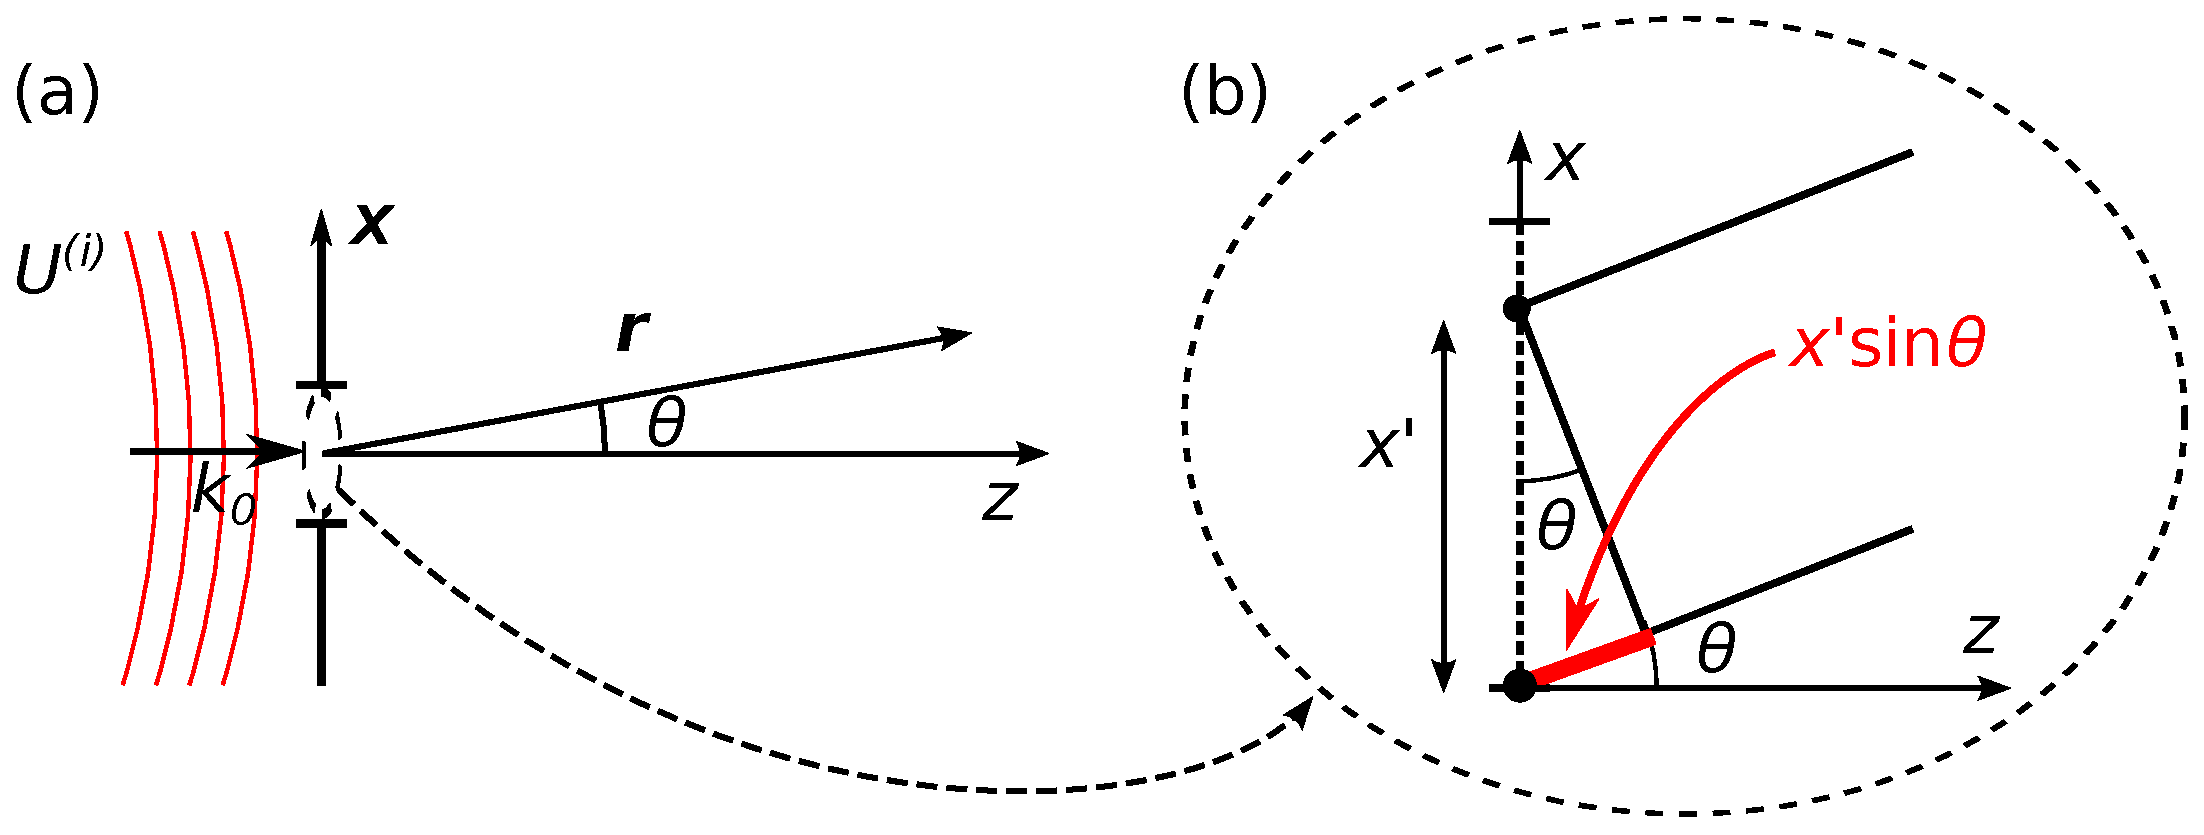
\includegraphics[width = \textwidth]{%
    Chapters/InterferometricMethods/figs/Fraunhofer_geometric_phase_factor.eps}
  \caption[Fraunhofer geometric phase factor]{%
    (a) Typical Fraunhofer diffraction geometry and
    (b) a close up that displays the path-length difference $x' \sin\theta$
    between a wave emanating from the origin and
    a wave emanating from $x'$}
\label{fig:InterferometricMethods:Fraunhofer_geometric_phase_factor}
\end{figure}


\subsection{Fraunhofer diffraction of a phase-modulated Gaussian beam}
Now, assume that the phase of the incident beam
is sinusoidally modulated at $S_1$ as
\begin{equation}
  \tilde{\phi}(x', t) = \tilde{\phi}_0 \cos(k x' - \omega t)
\end{equation}
This adds an additional phase contribution to
(\ref{eq:InterferometricMethods:Fraunhofer_diffraction_integral_free_space})
such that the diffraction pattern in the $x$-direction is given as
\begin{align}
  D_x
  &=
  \int_{-\infty}^{\infty}
  e^{-( x' / w_0 )^2}
  e^{-i k_0 x x' / r}
  e^{i \tilde{\phi}(x', t)}
  dx'
  \notag \\
  &=
  \int_{-\infty}^{\infty}
  e^{-( x' / w_0 )^2}
  e^{-i k_0 x x' / r}
  e^{i \tilde{\phi}_0 \cos(k x' - \omega t)}
  dx'
  \notag \\
  &=
  \int_{-\infty}^{\infty}
  e^{-( x' / w_0 )^2}
  e^{-i k_0 x x' / r}
  \left\{%
    \sum_{m = -\infty}^{\infty}
    i^m \left[ J_m(\tilde{\phi}_0) \right]
    e^{i m (k x' - \omega t)}
  \right\}
  dx'
  \notag \\
  &=
  \sum_{m = -\infty}^{\infty}
  i^m \left[ J_m(\tilde{\phi}_0) \right]
  e^{-i m \omega t}
  \int_{-\infty}^{\infty}
  e^{-( x' / w_0 )^2}
  e^{-i \left( \frac{k_0 x}{r} - m k \right) x'}
  dx'
  \notag \\
  &=
  \sqrt{\pi} w_0
  \sum_{m = -\infty}^{\infty}
  i^m \left[ J_m(\tilde{\phi}_0) \right]
  e^{-i m \omega t}
  e^{-\left[ \frac{w_0}{2} \left( \frac{k_0 x}{r} - m k \right) \right]^2}
  \label{eq:InterferometricMethods:Fraunhofer_diffraction_integral_phase_modulated}
\end{align}
where the expression in the third line follows from
application of the well-known Jacobi-Anger expansion, and
$J_m$ is the $m$\ts{th} Bessel function of the first kind.
Noting that $E(\vect{r}, t) = E(\vect{r}) e^{-i \omega_0 t}$,
substitution of
(\ref{eq:InterferometricMethods:Fraunhofer_diffraction_integral_phase_modulated})
into (\ref{eq:InterferometricMethods:Fraunhofer_diffracted_field}) yields
\begin{align}
  \begin{aligned}
    E(\vect{r}, t)
    \approx
    &\sum_{m = -\infty}^{\infty}
    i^m \left[ J_m(\tilde{\phi}_0) \right]
    e^{-i m \omega t}
    e^{-\left[ \frac{w_0}{2} \left( \frac{k_0 x}{r} - m k \right) \right]^2}
    \\
    &\times
    \left[
      -i E_0
      \left( \frac{z_R}{z} \right)
      e^{-(k_0 w_0 y / 2 r)^2}
      e^{i (k_0 r - \omega_0 t)}
    \right]
  \label{eq:InterferometricMethods:Fraunhofer_phase_modulated_Gaussian_beam_diffraction}
  \end{aligned}
\end{align}

\begin{figure}
  \centering
  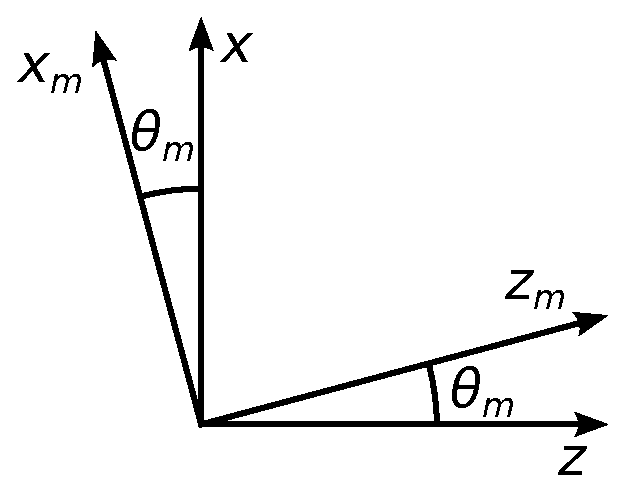
\includegraphics[width = 0.4 \textwidth]{%
    Chapters/InterferometricMethods/figs/coordinate_rotation.eps}
  \caption{Coordinate transformation for interpretation of
    the diffraction pattern of a phase-modulated Gaussian beam}
\label{fig:InterferometricMethods:coordinate_rotation}
\end{figure}

To put
(\ref{eq:InterferometricMethods:Fraunhofer_phase_modulated_Gaussian_beam_diffraction})
in a more familiar form,
consider the coordinate transformation
\begin{align}
  \begin{aligned}
    z &= z_m \cos\theta_m - x_m \sin\theta_m
    \\
    x &= x_m \cos\theta_m + z_m \sin\theta_m
  \end{aligned}
\end{align}
where
\begin{equation}
  \sin \theta_m
  \equiv
  \frac{m k}{k_0}
  \label{eq:InterferometricMethods:scattering_angles}
\end{equation}
This coordinate transformation is depicted graphically
in Fig.~\ref{fig:InterferometricMethods:coordinate_rotation}.
Note that the transformation preserves lengths, i.e.\ $r_m = r$.
Typically, $k / k_0 \ll 1$ such that
\begin{align}
  \begin{aligned}
    z &\approx z_m - x_m \theta_m
    \\
    x &\approx x_m + z_m \theta_m
  \end{aligned}
  \label{eq:InterferometricMethods:coordinate_rotation}
\end{align}
Substituting
(\ref{eq:InterferometricMethods:coordinate_rotation})
into
(\ref{eq:InterferometricMethods:Fraunhofer_phase_modulated_Gaussian_beam_diffraction})
and defining $\rho_m = (x_m^2 + y^2)^{1/2}$ yields
\begin{equation}
  \begin{aligned}
    E(\vect{r}, t)
    \approx
    &\sum_{m = -\infty}^{\infty}
    i^m \left[ J_m(\tilde{\phi}_0) \right]
    e^{-i (\omega_0 + m \omega) t}
    \\
    &\times
    \left[
      -i E_0
      \left( \frac{z_R}{z_m} \right)
      e^{-(k_0 w_0 \rho_m / 2 r)^2}
      e^{i k_0 r}
    \right]
  \end{aligned}
\end{equation}
where the far-field limit has been used to approximate $1/z \approx 1/z_m$.
Now, the bracketed expression has the form of
(\ref{eq:InterferometricMethods:Fraunhofer_Gaussian_beam_diffraction})
for a far-field Gaussian beam; thus,
the diffracted electric field can be more compactly and generally written as
\begin{equation}
  E(\vect{r}, t)
  \approx
  \sum_{m = -\infty}^{\infty}
  i^m \left[ J_m(\tilde{\phi}_0) \right]
  E_G(\vect{r_m})
  e^{-i (\omega_0 + m \omega) t}
  \label{eq:InterferometricMethods:Fraunhofer_phase_modulated_Gaussian_beam_diffraction_compact}
\end{equation}
where $\vect{r_m} \approx (x - z \theta_m,\, y,\, z + x \theta_m)$.
Note that
(\ref{eq:InterferometricMethods:Fraunhofer_phase_modulated_Gaussian_beam_diffraction_compact})
is valid for $0 \leq z < \infty$ rather than only for $z \gg z_R$;
that is, computing the far-field diffraction pattern
has additionally allowed inferring the corresponding near-field.

Thus, a sinusoidal phase modulation diffracts an incident Gaussian beam
into an infinite number of \emph{scattered} Gaussian beams.
The incident beam is coupled into the $m$\ts{th} scattered beam
with strength $J_m(\tilde{\phi}_0)$.
The $m$\ts{th} scattered beam is Doppler shifted
relative to the incident beam by $m \omega$ and
propagates at an angle $\theta_m \approx m k / k_0$
relative to the optical axis.
Note that the spatial dependence of the scattered beams' phase evolution
remains $e^{i [k_0 r - \psi(z)]}$; that is,
the scattering process is elastic,
with $|\vect{k^{(i)}}| = |\vect{k_m}| = k_0$.
This constraint of elasticity
coupled with knowledge of the scattering angle $\theta_m$
allows determination of the scattered wavevector
\begin{equation}
  \vect{k_m}
  =
  (m k) \hat{\vect{x}}
  +
  k_0 \left[ 1 - \left(\frac{m k}{k_0}\right)^2 \right]^{1/2} \hat{\vect{z}}
  %k_0 \sqrt{1 - \left(\frac{m k}{k_0}\right)^2} \hat{\vect{z}}
  \label{eq:InterferometricMethods:scattered_beam_wavevector}
\end{equation}
Obviously, the scalar nature of the above diffraction calculation
is insufficient to capture
the small polarization changes that accompany beam scattering.
However, the field must remain transverse.
Thus, if the incident beam polarization is
$\hat{\vect{e}}^{(i)}
=
(1 - p_y^2)^{1/2} \hat{\vect{x}}
+
p_y \hat{\vect{y}}$,
the polarization of the $m$\ts{th} scattered beam is
\begin{equation}
  \hat{\vect{e}}_m
  \approx
  \sqrt{\frac{1 - p_y^2}{1 + \theta_m^2}}
  \left( \hat{\vect{x}} - \theta_m \hat{\vect{z}} \right)
  +
  p_y \hat{\vect{y}}
  \label{eq:InterferometricMethods:scattered_beam_polarization}
\end{equation}


\subsection{Imaging of the scattered radiation}
It is often desirable to \emph{image} the above scattered radiation
in order to determine the spatiotemporal aspects
of the responsible phase fluctuations.
The optical axis of each scattered Gaussian beam
behaves as a ray in the geometric-optics sense
\cite{tovar_generalized_beam_matrices_IV}, and
an imaging system $\mathcal{I}$ redirects all such rays
emanating from position $\vect{\rho}$ in the object plane $S_1$
to intersect at position
$\vect{\rho'} = \mathcal{I}(\vect{\rho}) = M \vect{\rho}$ in the image plane.
Here, $M$ is the \emph{magnification} of the imaging system, and
$M < 0$ implies that the image is inverted relative to the object.
Thus, the phase-fluctuation wavevector $k$
is imaged as $k / M$ such that
the wavevector of the $m$\ts{th} scattered beam in the image plane is
\begin{align}
  \vect{k_m'}
  &=
  \mathcal{I}(\vect{k_m})
  =
  \left( \frac{m k}{M} \right) \hat{\vect{x}}
  +
  k_0 \left[ 1 - \left(\frac{m k}{M k_0}\right)^2 \right]^{1/2} \hat{\vect{z}}
  %k_0 \sqrt{1 - \left(\frac{m k}{k_0}\right)^2} \hat{\vect{z}}
  \label{eq:InterferometricMethods:scattered_beam_wavevector_image_plane}
\end{align}
and the $m$\ts{th} scattered beam is rotated by angle $\theta_m / M$
relative to the unscattered beam in the imaging plane,
as shown in Fig.~\ref{fig:InterferometricMethods:imaging_geometry}.

\begin{figure}
  \centering
  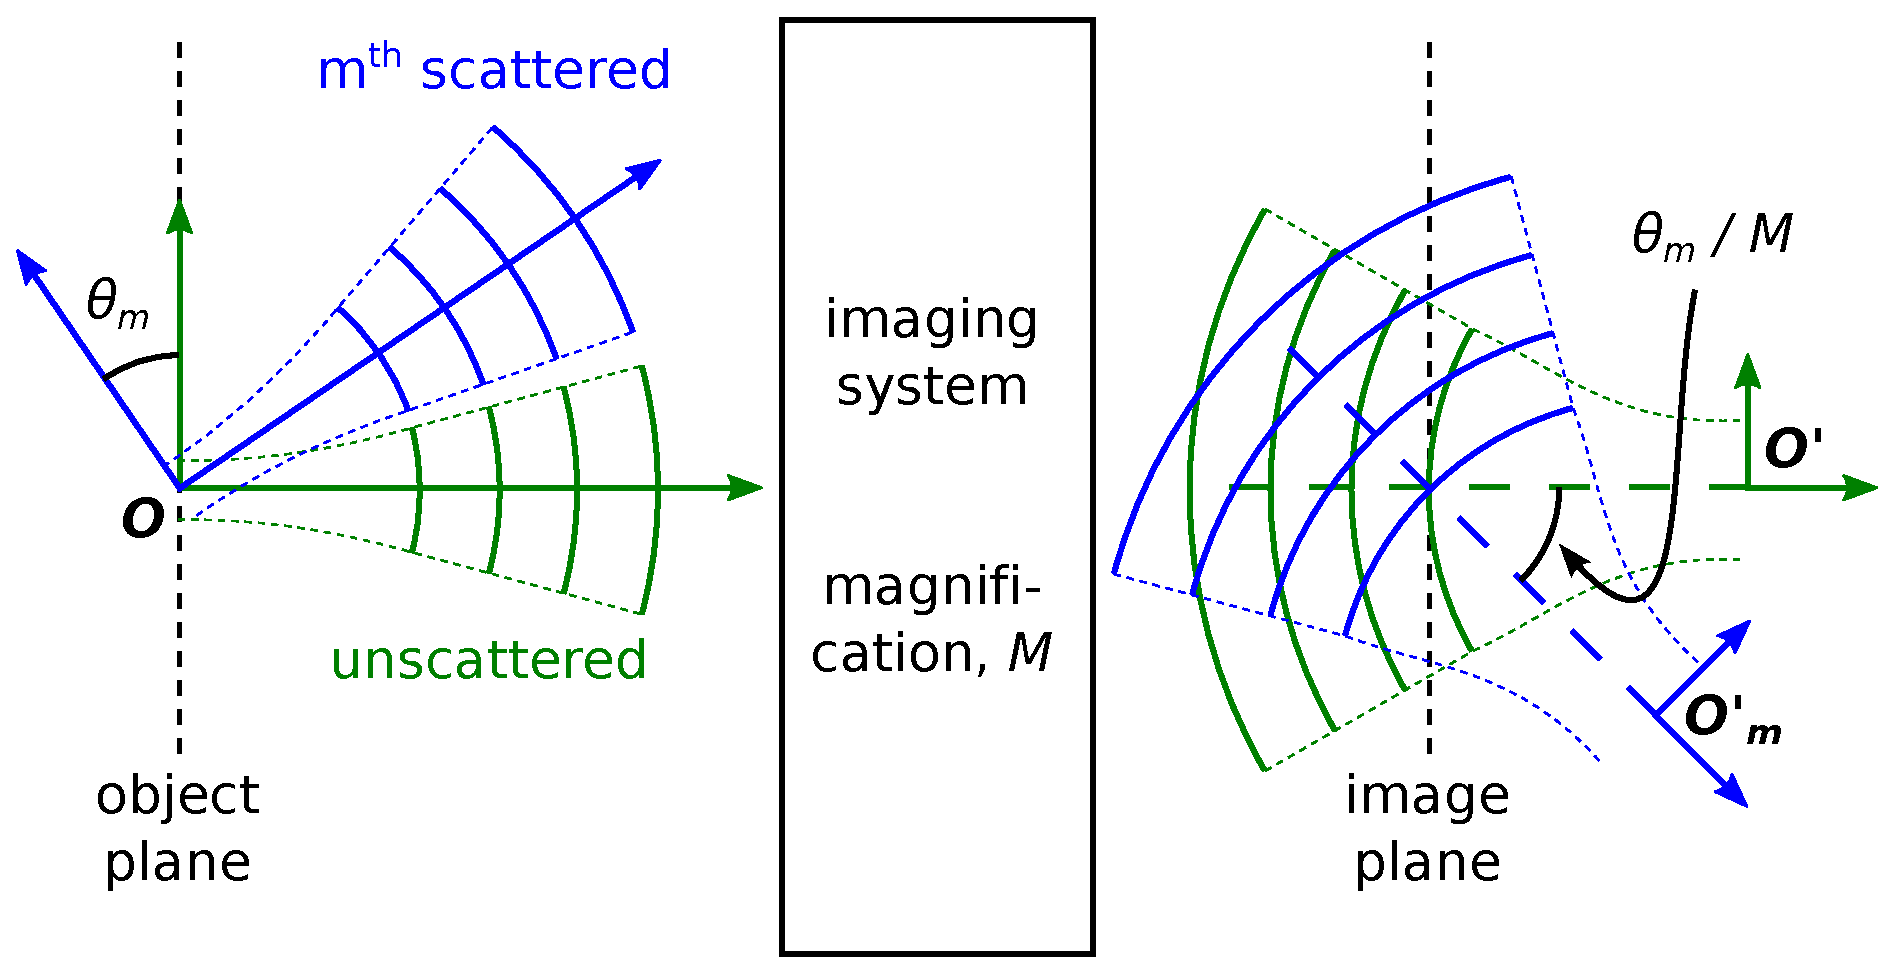
\includegraphics[width = \textwidth]{%
    Chapters/InterferometricMethods/figs/imaging_geometry.eps}
  \caption[Imaging geometry]{%
    Beam geometries in an imaging system with magnification $M$.
    Beam scattering occurs in the object plane at the probe beam's waist.
    Thus, the $m$\ts{th} scattered beam
    shares the origin $\vect{O}$ with the unscattered beam but
    is angularly separated by $\theta_m$.
    The imaging system redirects all beams emanating from $\vect{O}$
    to intersect at angle $\theta_m / M$ in the image plane.
    In general, the image plane does \emph{not} sit at a beam waist
    such that the post-imaging-system beam waists
    of the scattered and unscattered beams do not coincide,
    i.e.\ $\vect{O'} \neq \vect{O_m'}$.}
\label{fig:InterferometricMethods:imaging_geometry}
\end{figure}

The imaging optics also alter
the properties of the incident Gaussian beams.
In addition to its in-medium wavelength $\lambda_0 / N$,
a Gaussian beam is fully characterized by
its width $w(z_i)$ and
its radius of curvature $R(z_i)$
at a single location $z_i$.
The beam can then be propagated
forwards or backwards in a given optical train
using the corresponding ray matrices of geometric optics
\cite{siegman_lasers}.
Further, for a given optical train in the paraxial limit,
a Gaussian beam's width and radius of curvature evolve independently of
its transverse and angular displacements from
the optical train's nominal axis
\cite{tovar_generalized_beam_matrices_IV}.
That is, as any given scattered beam
propagates through an imaging system $\mathcal{I}$,
the evolution of its width and radius of curvature
will be \emph{identical} to that of the unscattered beam
propagating through the same imaging system.
However, the waists of the post-imaging-system beams
do \emph{not} necessarily sit at the image plane,
in which case the beams' native coordinate systems
are necessarily displaced from each other (i.e.\ $\vect{O'} \neq \vect{O'_m}$),
as indicated in Fig.~\ref{fig:InterferometricMethods:imaging_geometry}.

As will be demonstrated shortly,
the transformation between
the native coordinate system of the $m$\ts{th} scattered beam and
that of the unscattered beam in the image plane
is needed.
It may be useful to refer to
Fig.~\ref{fig:InterferometricMethods:coordinate_transformation_imaging_plane}
in the following discussion.
The coordinate transformation is easily found
through a series of translations and rotations.
Let point $P$ be represented
in the native coordinate system of the unscattered beam
by the ordered pair $(z_0', x_0')$.
Then, the representation of $P$ in the $\alpha$-base is
\begin{equation}
  \begin{pmatrix}
    z_{\alpha}' \\
    x_{\alpha}'
  \end{pmatrix}
  =
  \begin{pmatrix}
    z_0' - z' \\
    x_0'
  \end{pmatrix}
\end{equation}
The $\alpha$- and $\beta$-bases are related via a rotation
\begin{equation}
  \begin{pmatrix}
    z_{\beta}' \\
    x_{\beta}'
  \end{pmatrix}
  =
  \begin{pmatrix}
    \cos\left( \frac{\theta_m}{M} \right)
    &
    \sin\left( \frac{\theta_m}{M} \right)
    \\
    -\sin\left( \frac{\theta_m}{M} \right)
    &
    \cos\left( \frac{\theta_m}{M} \right)
  \end{pmatrix}
  \begin{pmatrix}
    z_{\alpha}' \\
    x_{\alpha}'
  \end{pmatrix}
\end{equation}
Finally, a linear translation converts the $\beta$-base
into the native coordinate system of the $m$\ts{th} scattered beam
in the image plane
\begin{equation}
  \begin{pmatrix}
    z_m' \\
    x_m'
  \end{pmatrix}
  =
  \begin{pmatrix}
    z_{\beta}' +  z' \\
    x_{\beta}'
  \end{pmatrix}
\end{equation}
Combining the above steps and
evaluating at the image plane ($z_0' = z', \, x_0' = x'$)
yields the image-plane coordinate transformation
\begin{equation}
  \begin{pmatrix}
    z_m' \\
    x_m'
  \end{pmatrix}
  =
  \begin{pmatrix}
    z' + x' \sin\left( \frac{\theta_m}{M} \right) \\
    x' \cos\left( \frac{\theta_m}{M} \right)
  \end{pmatrix}
  \approx
  \begin{pmatrix}
    z' + \left( \frac{m k}{M k_0} \right) x' \\
    x' - \frac{1}{2} \left( \frac{m k}{M k_0} \right)^2 x'
  \end{pmatrix}
  \label{eq:InterferometricMethods:coordinate_transformation_imaging_plane}
\end{equation}
where the approximation holds for
the typical small-angle scattering limit ($\theta_m \ll 1$).

\begin{figure}
  \centering
  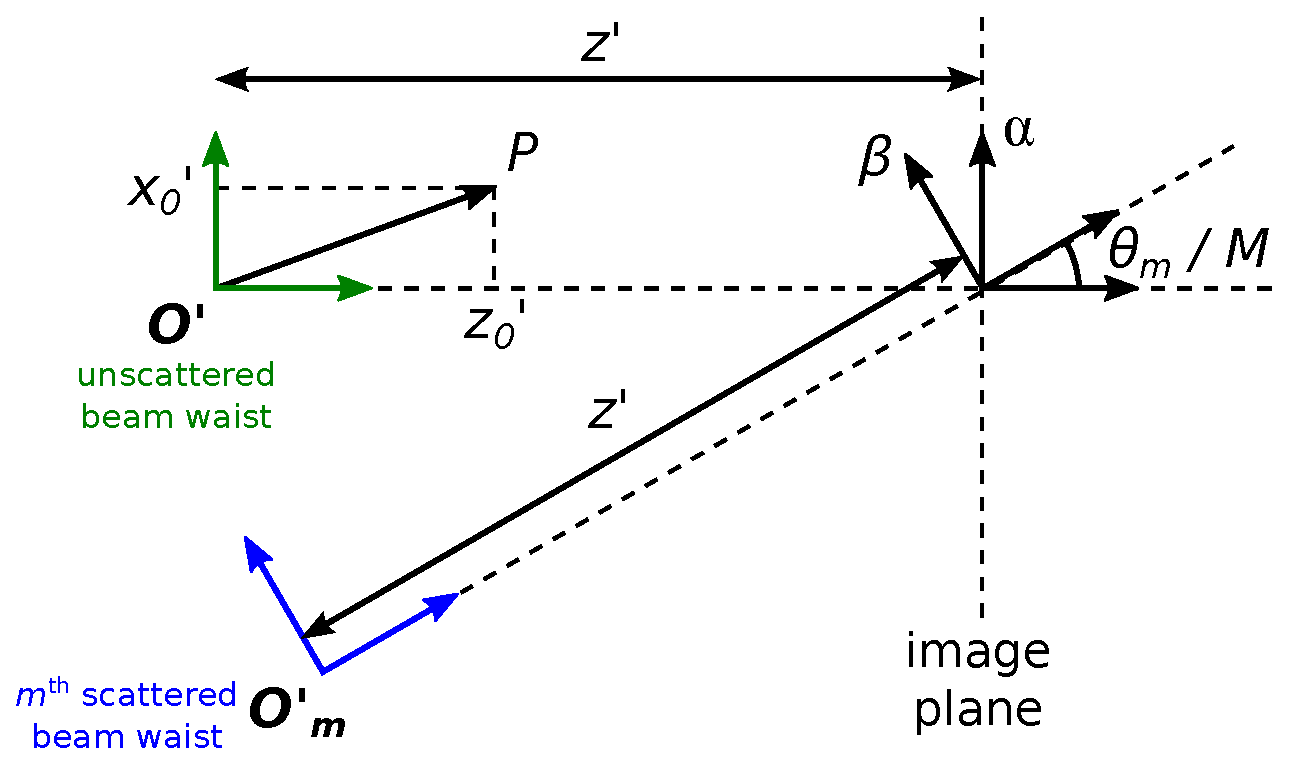
\includegraphics[width = 0.9 \textwidth]{%
    Chapters/InterferometricMethods/figs/coordinate_transformation_imaging_plane.eps}
  \caption[Imaging-plane coordinate transformation]{%
    Imaging-plane coordinate transformation}
\label{fig:InterferometricMethods:coordinate_transformation_imaging_plane}
\end{figure}

Now, without further ado,
let $\mathcal{I}$ image the object plane $S_1$
such that the image of diffracted field
(\ref{eq:InterferometricMethods:Fraunhofer_phase_modulated_Gaussian_beam_diffraction_compact})
is
\begin{equation}
  \mathcal{I}[ E(\vect{r}, t) ]
  =
  \sum_{m = -\infty}^{\infty}
  i^m \left[ J_m(\tilde{\phi}_0) \right]
  \mathcal{I}[E_G(\vect{r_m})]
  e^{-i (\omega_0 + m \omega) t}
\end{equation}
where the linearity of $\mathcal{I}$ has been invoked
to bring the operator within the summation.
The imaging optics simply transform
the $m$\ts{th} scattered Gaussian beam as
\begin{align}
  \mathcal{I}[E_G(\vect{r_m})]
  &=
  E_{G'}(\vect{r_m'})
  \notag \\
  &
  \begin{aligned}
    &= E_0
    \frac{w_0'}{w'(z_m')}
    \exp\left[ \frac{-\rho_m'^2}{w'(z_m')^2} \right]
    \\
    &\quad\times
    \exp\left\{ i \left[
      k_0 z_m'
      +
      \frac{k_0 \rho_m'^2}{2 R'(z_m')}
      -
      \psi'(z_m') \right] \right\}
  \end{aligned}
\end{align}
where $w'(z_m')$, $R'(z_m')$, and $\psi'(z_m')$ are the beam's image-plane
width, radius of curvature, and Gouy phase shift, respectively.
Under the typical small-angle scattering limit,
$w'(z_m') \approx w'(z')$,
$R'(z_m') \approx R'(z')$, and
$\psi'(z_m') \approx \psi'(z')$.
Then, neglecting the small variation in the Gaussian envelope and
retaining phase-factor terms only to second order in $k / k_0$,
the $m$\ts{th} scattered Gaussian beam in the image plane is
\begin{equation}
  \mathcal{I}[E_G(\vect{r_m})]
  =
  E_{G'}(\vect{r'})
  \exp\left\{%
    i \left[%
      \frac{m k x'}{M}
      -
      \frac{1}{2 k_0 R'(z')} \left( \frac{m k x'}{M} \right)^2
    \right]
  \right\}
  \label{eq:InterferometricMethods:imaged_scattered_beam_second_order}
\end{equation}
where
\begin{align}
  \begin{aligned}
    E_{G'}(\vect{r'})
    =
    &\, E_0
    \frac{w_0'}{w'(z')}
    \exp\left[ \frac{-\rho'^2}{w'(z')^2} \right]
    \\
    &\times
    \exp\left\{ i \left[
        k_0 z'
        +
        \frac{k_0 \rho'^2}{2 R'(z')}
        -
        \psi'(z')
      \right]
    \right\}
  \end{aligned}
  \label{eq:InterferometricMethods:eq:InterferometricMethods:imaged_unscattered_beam}
\end{align}
corresponds to the field pattern of the unscattered Gaussian beam
in the image plane.
The quadratic term in the phase factor of
(\ref{eq:InterferometricMethods:imaged_scattered_beam_second_order})
is typically negligible but can become important during calibrations
(\textcolor{red}{cite Naoto and Dorris. Or even save for later chapter?}).
In the remainder of this chapter's discussion,
the quadratic term in the phase factor is dropped.
Thus, the total scattered field in the image plane becomes
\begin{equation}
  \mathcal{I}[ E(\vect{r}, t) ]
  =
  \left[ E_{G'}(\vect{r'}) e^{-i \omega_0 t} \right]
  \sum_{m = -\infty}^{\infty}
  i^m \left[ J_m(\tilde{\phi}_0) \right]
  e^{i m \left( \frac{k x'}{M} - \omega t \right)}
  \label{eq:InterferometricMethods:imaged_total_field}
\end{equation}


\begin{itemize}
  \item Typical limit with $\tilde{\phi}_0 \ll 1$
\end{itemize}


\section{Laser-plasma interactions in a tokamak}
\begin{itemize}
  \item Cold-plasma dispersion relation and derivation of $N$
  \item Expected phase shifts in tokamak plasma
  \item Refraction
  \item Scattering/diffraction
\end{itemize}

\section{Interferometry}
\begin{itemize}
  \item Homodyne
  \item Heterodyne
  \item Vibrations
  \item $k$-response
\end{itemize}

\section{Phase contrast imaging}
\begin{itemize}
  \item Principle
  \item $k$-response
\end{itemize}


\bibliographystyle{plainurl}
\bibliography{references}
